%%%%%%%%%%%%%%%%%%%%%%%%%%%%%%%%%%%%%%%%%%%%%%%%%%%%%%%%%%%%%%%%%%%%%%%%%%%%%
% CS437/CS5317/EE414/EE513 — Deep Learning, Spring 2026
% Group 26 | Hassan Iftikhar (27100204) | Saim Bilal (27100208)
%%%%%%%%%%%%%%%%%%%%%%%%%%%%%%%%%%%%%%%%%%%%%%%%%%%%%%%%%%%%%%%%%%%%%%%%%%%%%

\documentclass{article}

\usepackage{microtype}
\usepackage{graphicx}
\usepackage{subfigure}
\usepackage{booktabs}
\usepackage{amsmath}
\usepackage{amssymb}
\usepackage{hyperref}
\usepackage{multirow}
\usepackage{array}
\usepackage{placeins}

\newcommand{\theHalgorithm}{\arabic{algorithm}}

\usepackage[accepted]{icml2021}

\icmltitlerunning{Morphologically Grounded ECG Classification}

\begin{document}

\twocolumn[
\icmltitle{Morphologically Grounded ECG Arrhythmia Classification:\\
A Progressive CNN Pipeline with Physiological Alignment Supervision}

\begin{icmlauthorlist}
\icmlauthor{Hassan Iftikhar (27100204)}{}
\icmlauthor{Saim Bilal (27100208)}{}
\end{icmlauthorlist}

\icmlkeywords{ECG classification, morphological grounding, physiological alignment, explainability, PTB-XL}

\vskip 0.3in

\textbf{GitHub:} \url{https://github.com/hassan7-dev/ecg-morphological-grounding-dl-project.git}
\vskip 0.1in
]

%--------------------------------------------------------------------
\begin{abstract}
Deep ECG classifiers routinely achieve high benchmark accuracy by
latching on to amplitude statistics and recording-level shortcuts
rather than the localised wave morphology that cardiologists actually
inspect. This paper works through the problem in three stages on
PTB-XL, restricted to Leads~ I, II, and VI, and five diagnostic superclasses. We
first establish a 1D-ResNet baseline with Butterworth-filtered inputs
and measure saliency quality through a Morphological Alignment Score
(MAS) computed against NeuroKit2-derived P/QRS/T boundaries. The
first improvement runs a five-condition preprocessing ablation: we
designed Lead-wise Beat-Warp Augmentation (LBWA), a beat-preserving
augmentation grounded in both the STAR framework and piecewise time-warping
theory, but the ablation showed that raw ECG with z-score normalisation
alone outperforms every filtered or augmented variant on Macro-AUC,
Macro-F1, and MAS. Building on that finding, the second improvement
keeps the raw-signal pipeline and adds class-conditioned physiological
alignment supervision, which regularises the model's class activation
maps toward Gaussian priors encoding the diagnostically relevant wave
regions for each arrhythmia. The Full alignment model improves
class-specific MAS by 58\% relative to the raw-signal baseline with
a marginal gain in Macro-AUC (0.8960 $\to$ 0.8968), and the
Conduction Disturbance class, whose defining feature is QRS widening,
sees a tenfold increase in region-specific MAS.
\end{abstract}

%--------------------------------------------------------------------
\section{Introduction}

The 12-lead electrocardiogram remains the default first test in cardiac
workups, and for good reason: arrhythmias leave specific, readable
fingerprints on the waveform. Wolff-Parkinson-White produces a delta
wave before the QRS complex. Long QT syndrome extends the QT interval
beyond 480\,ms. Atrial fibrillation replaces organised P-waves with
irregular RR intervals. A cardiologist works through these cues
sequentially: inspect the P-wave, measure the PR interval, examine
QRS width, then read the ST segment and T-wave.

Deep networks, by contrast, appear to skip this entirely. Ansari et
al.~\cite{ansari2023} surveyed 368 deep learning studies from 2017 to
2023 and found that benchmark Macro-F1 scores are routinely driven by
spectral envelopes and amplitude statistics, not the specific
morphological intervals that carry diagnostic meaning. Three failure
modes compound one another: shortcut learning (majority-class texture
dominates gradient attribution), augmentation-morphology conflict
(global time-warping distorts PR intervals and QT durations as if
stretching artefact mimics pathology), and physiologically naive
denoising (Butterworth bandpass filters attenuate the low-frequency
P-wave envelope, degrading exactly the feature needed for
P-wave-dependent diagnoses).

Our work does not try to match the full complexity of a cardiologist's
reasoning process. The narrower aim is to ask whether we can at least
align the model's spatial attention with the ECG regions a clinician
would look at to justify a given prediction. We quantify this through
a Morphological Alignment Score applied at two levels of granularity
across three progressive stages.

The specific contributions are:
\begin{itemize}
  \item A five-condition preprocessing ablation that includes an
    honest negative result: LBWA, a beat-preserving augmentation
    we designed by combining the STAR principle with piecewise
    time-warping theory~\cite{iwana2021}, consistently hurt both
    classification accuracy and morphological alignment compared
    to the no-augmentation baseline, while raw ECG with z-score
    normalisation won across every metric.
  \item A class-conditioned physiological alignment supervision
    framework that regularises class activation maps toward
    Gaussian priors encoding the diagnostically relevant wave
    regions per arrhythmia class, improving class-specific MAS
    by 58\% with minimal classification cost.
  \item An empirical finding that Butterworth filtering, despite
    being standard practice, measurably suppresses morphological
    learning compared to processing the raw signal.
\end{itemize}

%--------------------------------------------------------------------
\section{Related Work}

\textbf{Surveys and the morphology gap.}
The most complete picture of where the field stands comes from
Ansari et al.~\cite{ansari2023}, whose review of 368 studies
establishes that 1D CNNs dominate (59\% of architectures) and only
28\% of studies apply any augmentation at all, let alone
morphology-aware augmentation. Crucially, none evaluated whether
their augmentation preserved the P-QRS-T ordering that clinical
diagnosis depends on.

\textbf{Explainability baselines.}
Talukder et al.~\cite{talukder2025} provide the most directly useful
calibration point: their Grad-CAM maps localise to the QRS complex
for ventricular arrhythmias and to the P-wave region for
supraventricular classes. We adopt this localisation pattern as the
qualitative target for our MAS metric. Pantelidis et
al.~\cite{pantelidis2025} release open-source Grad-CAM code and
pre-trained PTB-XL weights for a multi-scale Inception-1D baseline,
which we use as a post-hoc XAI reference. The practical upper bound
on intrinsic explainability is set by ProtoECGNet~\cite{sethi2025},
a prototype-based architecture that justifies predictions via
similarity to learned beat exemplars.

\textbf{Architecture for morphology.}
Hammer et al.~\cite{hammer2024} separate a short morphology branch
(0.6\,s windows) from a long rhythm branch (10\,s windows) in their
xECGArch, validating separation via pixel-flipping. That
morphology-rhythm distinction informs the design of our physiological
priors, even though we pursue it through a loss-function approach
rather than a dual-branch architecture.

\textbf{Denoising.}
The Stationary Wavelet Transform with a Daubechies-8 wavelet
is theoretically superior to Butterworth bandpass for preserving
P-wave amplitude, because it operates on frequency bands in a
shift-invariant way without the subsampling artefacts of the
discrete wavelet transform~\cite{addison2005,lee2019}. We tested
this empirically and the results are in Section~\ref{sec:task4}.

\textbf{Augmentation.}
Nemati~\cite{nemati2025} introduced STAR, which applies sinusoidal
time-amplitude resampling within each RR interval to simulate heart
rate variability without distorting intra-beat morphology. STAR
was not peer-reviewed at the time of writing, so we grounded our
LBWA design additionally in Iwana and Uchida~\cite{iwana2021}, whose
empirical study on 128 time-series datasets confirmed that piecewise
warping preserves class-discriminative structure better than global
warping.

%--------------------------------------------------------------------
\section{Methodology}

\subsection{Dataset and Evaluation Protocol}

All experiments use PTB-XL~\cite{strodthoff2021}, a dataset of
21,799 10-second 12-lead recordings at 500\,Hz. We restrict to Lead~I, II and IV
(indices~0, 1 and 6) and the five diagnostic superclasses: NORM, MI, STTC, CD,
and HYP. Table~\ref{tab:dataset} shows the class distribution.

\begin{table}[h!]
\caption{PTB-XL diagnostic superclass distribution (filtered dataset).}
\label{tab:dataset}
\vskip 0.1in
\begin{center}
\begin{small}
\begin{tabular}{lrr}
\toprule
Class & Records & \% of set \\
\midrule
NORM (Normal)               & 9,528 & 44.5 \\
MI (Myocardial Infarction)  & 5,486 & 25.6 \\
STTC (ST/T Change)          & 5,123 & 23.9 \\
CD (Conduction Disturbance) & 4,907 & 22.9 \\
HYP (Hypertrophy)           & 2,655 & 12.4 \\
\midrule
\multicolumn{3}{l}{Train/Val/Test splits: 17100 / 2155 / 2162} \\
\bottomrule
\end{tabular}
\end{small}
\end{center}
\end{table}

The canonical PTB-XL inter-patient split assigns folds 1--8 to
training, fold 9 to validation, and fold 10 to test. Patient-ID
intersection between training and test was verified to be zero before
each run. Raw accuracy is not reported; NORM exceeds 44\% of records
and accuracy would be trivially inflated by majority-class bias.
The primary metrics are Macro-AUC and Macro-F1.

\subsection{The Morphological Alignment Score}

We use two variants of the MAS across the three tasks, because the
second improvement introduces class-specific masks that are not
available in the simpler binary form.

\textbf{MAS\textsubscript{eval}} (Tasks 3 and 4) measures how much of a
Grad-CAM heatmap $H \in [0,1]^T$ falls within a binary
morphological mask $M \in \{0,1\}^T$ built by NeuroKit2's
\texttt{ecg\_delineate} function~\cite{makowski2021,pantompkins1985}
using Pan-Tompkins R-peak detection on Lead~II:
\begin{equation}
\mathrm{MAS_{eval}} = \frac{\sum_t H_t \cdot M_t}{\sum_t H_t + \varepsilon}.
\label{eq:mas_eval}
\end{equation}
A value near 1.0 indicates the heatmap is concentrated inside
P-wave, QRS, and T-wave windows; values near zero indicate the model
is attending to isoelectric baseline regardless of the predicted
class.

\textbf{MAS\textsubscript{physio}} (Task 5) replaces the binary NeuroKit2
mask with class-conditioned Gaussian soft priors derived from
class-specific wave weights, averaged over the full test population.
This is necessary because the alignment supervision framework
introduces per-class physiological targets that the binary mask
cannot distinguish. The two metrics are therefore not directly
comparable; Section~\ref{sec:task5} defines MAS\textsubscript{physio}
precisely.

\subsection{Task 3: Baseline Pipeline}
\label{sec:task3}

\textbf{Preprocessing.}
Three leads are used in the baseline: Lead~I (index 0), Lead~II
(index 1), and V1 (index 6). Each lead is independently filtered
with a third-order zero-phase Butterworth bandpass at 0.5--40\,Hz
and then Z-score normalised per recording. The three-lead design is
intentional: Lead~II provides the clearest P-wave axis, Lead~I
captures lateral ST changes, and V1 gives access to RBBB/LBBB
morphology and posterior MI patterns.

\textbf{Architecture.}
The backbone is an 18-layer-style 1D-ResNet. A stem convolution
(kernel size 15, stride 2) projects the input from 3 channels to 32
and halves the temporal dimension to 2500. Four progressive stages
of residual blocks follow:
\begin{itemize}
  \item Stage 1: $2 \times$ ResBlock$(32\to32, k=15)$ $\to (B, 32, 2500)$
  \item Stage 2: $2 \times$ ResBlock$(32\to64, k=15, s=2)$ $\to (B, 64, 1250)$
  \item Stage 3: $2 \times$ ResBlock$(64\to128, k=7, s=2)$ $\to (B, 128, 625)$
  \item Stage 4: $2 \times$ ResBlock$(128\to256, k=7, s=2)$ $\to (B, 256, 313)$
\end{itemize}
Stages 1 and 2 use $k{=}15$ (30\,ms at 500\,Hz) to capture steep P-wave
and R-peak slopes at high resolution; stages 3 and 4 use $k{=}7$
where the effective receptive field already spans $\approx$224\,ms,
enough for rhythm context. Global average pooling and a two-layer MLP
with sigmoid output produce the five-class multi-label prediction.

\textbf{Training.}
Binary cross-entropy with per-class positive weight
$w_c = N^{-}_c / N^{+}_c$ is used to counteract class imbalance.
AdamW (lr$=10^{-3}$, wd$=10^{-4}$) with ReduceLROnPlateau
(patience 5, factor 0.1, monitor val Macro-AUC) trains for 70 epochs;
best checkpoint is selected by validation Macro-AUC.

\textbf{Grad-CAM and MAS\textsubscript{eval}.}
Grad-CAM is applied to the last convolutional layer of stage~4. The
algorithm backpropagates the logit for class $c$, computes importance
weights $\alpha^c_k = \frac{1}{T}\sum_t \frac{\partial y^c}{\partial A^k_t}$,
and forms the heatmap $L^c = \mathrm{ReLU}(\sum_k \alpha^c_k A^k)$.
The heatmap is linearly upsampled from 313 to 5000 samples and
normalised to $[0,1]$ before MAS\textsubscript{eval} is computed
against the NeuroKit2 mask on Lead~II using Eq.~\ref{eq:mas_eval}.

\subsection{Task 4: Preprocessing Ablation and LBWA}
\label{sec:task4}

\textbf{LBWA design.}
We designed Lead-wise Beat-Warp Augmentation to address the
shortcoming identified in the SoA survey: standard augmentations
either corrupt beat morphology (Gaussian noise) or warp the entire
recording, which simultaneously and incorrectly stretches the PR
interval, QRS duration, and QT interval. The design draws on two
sources: the STAR principle of Nemati~\cite{nemati2025}, which
restricts augmentation to individual RR segments, and the empirical
validation by Iwana and Uchida~\cite{iwana2021} that piecewise
warping preserves class-discriminative structure in time-series data.

For each validated RR segment $i$, LBWA samples a warp factor
$c_i \sim \mathcal{U}(1-\alpha, 1+\alpha)$ with $\alpha{=}0.12$
and an amplitude factor $a_i \sim \mathcal{N}(1.0, 0.05)$. The
segment is resampled to the warped length and back, preserving global
signal length:
\begin{equation}
x'_i(t) = a_i \cdot c_i \cdot x_i\!\left(\frac{t}{c_i}\right),
\quad t \in [R_i, R_{i+1}].
\label{eq:lbwa}
\end{equation}
R-peaks are identified by a multi-lead majority vote (Pan-Tompkins
on each of the three leads via NeuroKit2; peaks confirmed by at least
two leads are retained). Any augmented beat that fails a morphological
fidelity check (P-QRS-T landmark count and ordering, up to 8 retries)
is rejected and resampled. LBWA is applied only to minority classes
(MI, STTC, CD, HYP).

\textbf{SWT denoising.}
The SWT pipeline decomposes each lead with a Daubechies-8 wavelet
at $J{=}8$ levels:
\begin{equation}
x(t) = a_J(t) + \sum_{j=1}^{J} d_j(t).
\label{eq:swt}
\end{equation}
The approximation $a_8$ (baseline wander $<$ 0.5\,Hz) is zeroed;
the detail $d_1$ (50\,Hz powerline band) is soft-thresholded with
a SURE threshold $\lambda = \hat{\sigma}\sqrt{2 \log N}$ where
$\hat{\sigma} = \mathrm{median}(|d_1|)/0.6745$. The SWT is
shift-invariant, avoiding the R-peak jitter introduced by
sub-sampling in the standard DWT~\cite{addison2005}.

\textbf{Morphological fidelity.}
Table~\ref{tab:fidelity} reports the fidelity check on 50 samples
(10 per class). The SWT satisfies the R-peak shift threshold
($<$1 sample) and R-peak sharpness retention ($>$90\%) but does not
achieve the 95\% P-wave amplitude retention target, nor does
Butterworth. This already hints that neither filter fully preserves
the low-amplitude P-wave envelope --- a result confirmed by the
ablation.

\begin{table}[h!]
\caption{Morphological fidelity: Butterworth vs SWT denoising.
Thresholds: R-shift $<$1 sample; P-retention $>$95\%; Sharpness $>$90\%.}
\label{tab:fidelity}
\vskip 0.1in
\begin{center}
\begin{small}
\begin{tabular}{lrrr|rrr}
\toprule
& \multicolumn{3}{c|}{Butterworth} & \multicolumn{3}{c}{SWT} \\
Class & Shift & P-ret & Sharp & Shift & P-ret & Sharp \\
\midrule
NORM & 0.08 & 54.3 & 62.7 & 0.03 & 52.6 & 96.4 \\
MI   & 0.18 & 61.8 & 60.4 & 0.06 & 58.2 & 96.2 \\
STTC & 0.10 & 68.3 & 77.3 & 0.00 & 67.7 & 96.5 \\
CD   & 0.17 & 63.9 & 59.9 & 0.03 & 61.7 & 98.1 \\
HYP  & 0.10 & 65.8 & 67.6 & 0.03 & 66.5 & 98.2 \\
Mean & 0.13 & 62.8 & 65.6 & 0.03 & 61.3 & 97.1 \\
\bottomrule
\end{tabular}
\end{small}
\end{center}
\end{table}

\textbf{Ablation conditions.}
The same 1D-ResNet architecture and training procedure from Task~3
is held fixed. Five preprocessing conditions vary only the denoising
and augmentation:
\textbf{A} -- Butterworth, no augmentation;
\textbf{B} -- Butterworth $+$ LBWA;
\textbf{C} -- SWT, no augmentation;
\textbf{D} -- SWT $+$ LBWA;
\textbf{E} -- raw ECG with z-score normalisation only (no filter, no augmentation).
Condition E serves as the lower-bound sanity check in the original
design but ended up winning on all metrics.

\subsection{Task 5: Physiological Alignment Supervision}
\label{sec:task5}

Given that raw ECG with z-score normalisation produced the best
MAS\textsubscript{eval}, Task~5 keeps that preprocessing and focuses
entirely on the training objective. The core question is whether
explicitly regularising the model's class activation maps toward
physiologically meaningful ECG regions improves alignment without
meaningfully sacrificing classification performance.

\textbf{Class activation maps.}
The backbone's \texttt{forward} pass is modified to expose the
pre-GAP feature map $F \in \mathbb{R}^{B \times C \times T'}$.
Class-specific CAMs are computed inline during training as:
\begin{equation}
\mathrm{CAM}[b,k,t] = \mathrm{ReLU}\!\left(\sum_c W_k^c \cdot F_{b,c,t}\right),
\label{eq:cam}
\end{equation}
where $W \in \mathbb{R}^{K \times C}$ is the classifier weight matrix.
Each CAM is normalised to a probability distribution over time. This
is far cheaper than Grad-CAM during training and produces the same
class-specific spatial maps.

\textbf{Class-conditioned physiological priors.}
Each wave region (P, QRS, ST, T) is represented as a Gaussian soft
mask centred at a fixed offset from the detected R-peak:
\begin{equation}
g(t; \mu, \sigma) = \exp\!\left(-\frac{(t-\mu)^2}{2\sigma^2}\right).
\label{eq:gauss}
\end{equation}
Offsets and widths encode typical inter-beat timing at 500\,Hz
(P: $-160$\,ms, $\sigma{=}60$\,ms; QRS: $0$\,ms, $\sigma{=}40$\,ms;
ST: $+120$\,ms, $\sigma{=}60$\,ms; T: $+280$\,ms, $\sigma{=}100$\,ms).
The combined prior for class $k$ is a weighted sum of wave masks,
downsampled to $T'$ and normalised:
\begin{equation}
\pi_k(t) \propto \sum_{w \in \{P,\,\mathrm{QRS},\,\mathrm{ST},\,T\}} \rho^w_k \cdot g(t;\mu_w,\sigma_w),
\label{eq:prior}
\end{equation}
where $\rho^w_k$ are class-wave weights encoding clinical knowledge.
For example, CD (QRS widening) uses $\rho^{\mathrm{QRS}}_{\mathrm{CD}}{=}1.0$
and zero elsewhere; STTC uses $\rho^{\mathrm{ST}}_{\mathrm{STTC}}{=}0.5$,
$\rho^{T}_{\mathrm{STTC}}{=}0.5$.

\textbf{MAS\textsubscript{physio}.}
For class $k$, the class-specific MAS is:
\begin{equation}
\mathrm{MAS}_{\mathrm{physio},k} = \mathbb{E}\!\left[\mathrm{CAM}_k \cdot \pi_k\right],
\label{eq:masphysio}
\end{equation}
averaged over the test population. Because $\pi_k$ is a narrow
Gaussian-weighted distribution, absolute values are small; the
relevant comparison is between ablation conditions.

\textbf{Four-term alignment loss.}
Let $\mathrm{CAM}_{\mathrm{act}}$ denote the stacked CAMs for
the active (label$=1$) classes in a batch, and $\pi_{\mathrm{act}}$
their corresponding priors. The total loss is:
\begin{equation}
\mathcal{L} = \mathcal{L}_{\mathrm{cls}}
+ \lambda_a \cdot \mathrm{conf} \cdot \mathcal{L}_{\mathrm{align}}
+ \lambda_o \cdot \mathrm{conf} \cdot \mathcal{L}_{\mathrm{out}}
+ \lambda_e \cdot \mathcal{L}_{\mathrm{entropy}},
\label{eq:loss}
\end{equation}
where $\mathcal{L}_{\mathrm{cls}}$ is binary cross-entropy with
per-class positive weights, and $\mathrm{conf}$ is the delineation
confidence score returned during mask pre-computation (poor-quality
masks produce weak rather than incorrect supervision).

$\mathcal{L}_{\mathrm{align}}$ is an asymmetric KL divergence:
\begin{equation}
\mathcal{L}_{\mathrm{align}} = \alpha\,\mathrm{KL}(\mathrm{CAM}\,\|\,\pi)
+ (1-\alpha)\,\mathrm{KL}(\pi\,\|\,\mathrm{CAM}),
\label{eq:align}
\end{equation}
with $\alpha{=}0.7$. The mode-seeking term $\mathrm{KL}(\mathrm{CAM}\,\|\,\pi)$
carries more weight because pure mean-seeking KL produces negligible
gradient when the CAM is initially diffuse, which is exactly when the
alignment signal is most needed.

$\mathcal{L}_{\mathrm{out}}$ penalises CAM mass outside the
physiological region:
\begin{equation}
\mathcal{L}_{\mathrm{out}} = \mathbb{E}[\mathrm{CAM} \cdot \mathbf{1}_{\mathrm{outside}}],
\label{eq:out}
\end{equation}
where ``outside'' is defined as the bottom $(1-q)$ timesteps by
prior probability with $q{=}0.35$.

$\mathcal{L}_{\mathrm{entropy}} = -\mathbb{E}[\mathrm{CAM} \cdot \log\mathrm{CAM}]$
sharpens temporal localisation by minimising entropy.

A linear warmup keeps all $\lambda$ values at zero for the first
few epochs while early CAMs stabilise. Only active classes
contribute to alignment losses; negative labels have no physiological
target to align toward.

\textbf{Ablation conditions.} Four conditions are trained on the same
raw $+$ z-score data and the same model:
\textbf{Baseline} ($\mathcal{L}_{\mathrm{cls}}$ only),
\textbf{Align} ($+\mathcal{L}_{\mathrm{align}}$),
\textbf{Align$+$Out} ($+\mathcal{L}_{\mathrm{align}}+\mathcal{L}_{\mathrm{out}}$),
\textbf{Full} (all four terms).

%--------------------------------------------------------------------
\section{Results}

\subsection{Task 3: Baseline Performance}

The baseline 1D-ResNet trained on Butterworth-filtered three-lead
inputs converges steadily over 70 epochs. Grad-CAM maps on the test
set show partial localisation to the QRS complex across most
superclasses, with weaker, less consistent localisation to P-wave
and ST-segment regions for CD and STTC respectively.
MAS\textsubscript{eval} for the Butterworth no-augmentation
condition (Condition~A from Task~4, which replicates the baseline
preprocessing) is reported in Table~\ref{tab:ablation}.

\subsection{Task 4: Preprocessing Ablation}

Table~\ref{tab:ablation} shows the five-condition results. Several
findings are worth noting directly.

First, raw ECG beats every filtered variant on all three metrics.
The gap is most pronounced in MAS\textsubscript{eval}: 0.711 for
raw versus 0.591 for SWT-only and 0.478 for Butterworth-only. This
is not a small margin.

Second, LBWA hurt performance in both filtering regimes. Butterworth$+$LBWA
dropped MAS\textsubscript{eval} from 0.478 to 0.456 compared to
Butterworth alone; SWT$+$LBWA dropped from 0.620 to 0.535. LBWA
also reduced Macro-F1 in both cases. Given this consistent negative
result, LBWA is dropped and raw$+$z-score is carried forward.

Third, the per-class breakdown reveals that MI and HYP benefit the
most from raw preprocessing in terms of AUC (0.909 and 0.818
respectively for Condition~E), while CD benefits most in
MAS\textsubscript{eval} under raw signals. Figures~\ref{fig:gradcam_A}
and~\ref{fig:gradcam_E} show the Grad-CAM overlays for Conditions~A
and~E respectively; the improvement in heatmap-mask overlap is
visible across MI, STTC, and CD.

\begin{table*}[t]
\caption{Five-condition preprocessing ablation (Task~4). MAS\textsubscript{eval}
computed via Grad-CAM vs.\ NeuroKit2 binary P/QRS/T mask. Best result per column
in bold.}
\label{tab:ablation}
\vskip 0.1in
\begin{center}
\begin{small}
\begin{tabular}{llrrrrrrrr}
\toprule
Cond. & Preprocessing & Macro-AUC & Macro-F1 & MAS\textsubscript{eval}
      & $\text{AUC}_\text{N}$ & $\text{AUC}_\text{MI}$ & $\text{AUC}_\text{STTC}$
      & $\text{AUC}_\text{CD}$ & $\text{AUC}_\text{HYP}$ \\
\midrule
A & Butterworth, no aug  & 0.8975 & \textbf{0.6952} & 0.478 & 0.929 & 0.906 & 0.915 & 0.924 & 0.814 \\
B & Butterworth + LBWA   & 0.8946 & 0.6722 & 0.456 & 0.931 & 0.896 & 0.911 & 0.921 & 0.814 \\
C & SWT, no aug          & 0.8984 & 0.6840 & 0.620 & 0.931 & \textbf{0.912} & 0.913 & \textbf{0.927} & 0.809 \\
D & SWT + LBWA           & 0.8931 & 0.6582 & 0.535 & 0.924 & 0.901 & 0.914 & 0.915 & 0.812 \\
\textbf{E} & \textbf{Raw + Z-score, no aug} & \textbf{0.8987} & 0.6949 & \textbf{0.711} & 0.930 & 0.909 & \textbf{0.916} & 0.919 & \textbf{0.818} \\
\bottomrule
\end{tabular}
\end{small}
\end{center}
\end{table*}

\begin{figure*}[t]
\centering
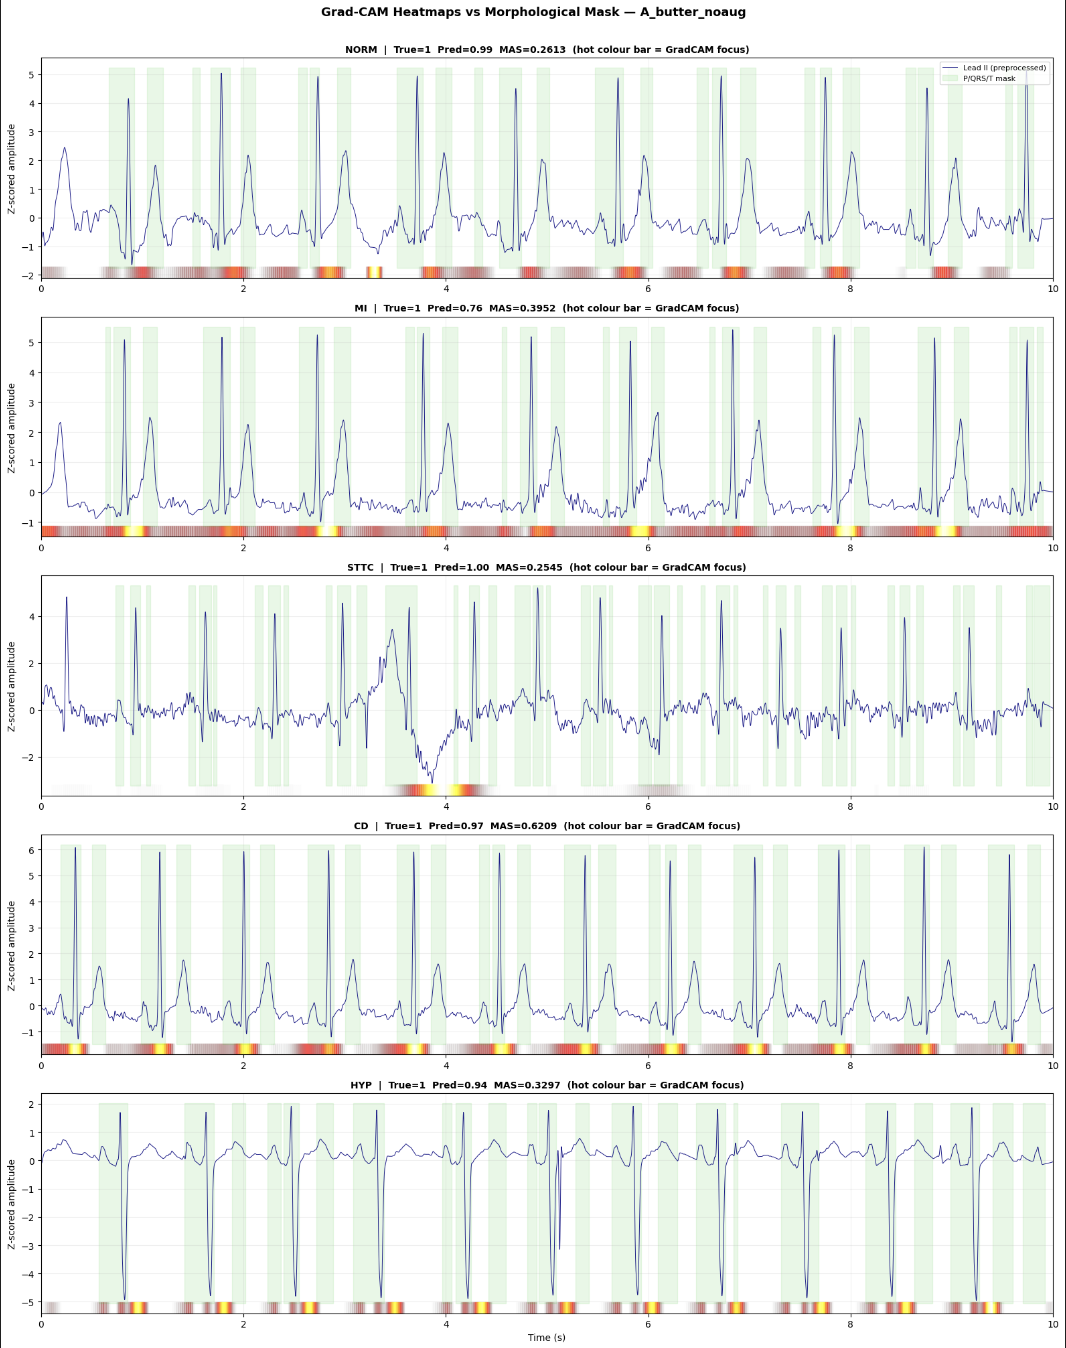
\includegraphics[width=0.78\textwidth]{gradcam_A.png}
\caption{\textbf{Condition A (Butterworth filter, no augmentation) — all five superclasses.}
Grad-CAM heatmaps overlaid on Lead~II. Hot colourbar at the bottom of each
panel marks where the model concentrates attention; green shading marks the
NeuroKit2-derived P/QRS/T morphological mask. Per-class MAS\textsubscript{eval}:
NORM = 0.261, MI = 0.395, STTC = 0.255, CD = 0.621, HYP = 0.330 (mean = 0.478).
The model attends largely to the high-amplitude QRS complex and isoelectric
baseline, with weak signal in the ST and P-wave windows for MI and STTC.}
\label{fig:gradcam_A}
\end{figure*}

\begin{figure*}[t]
\centering
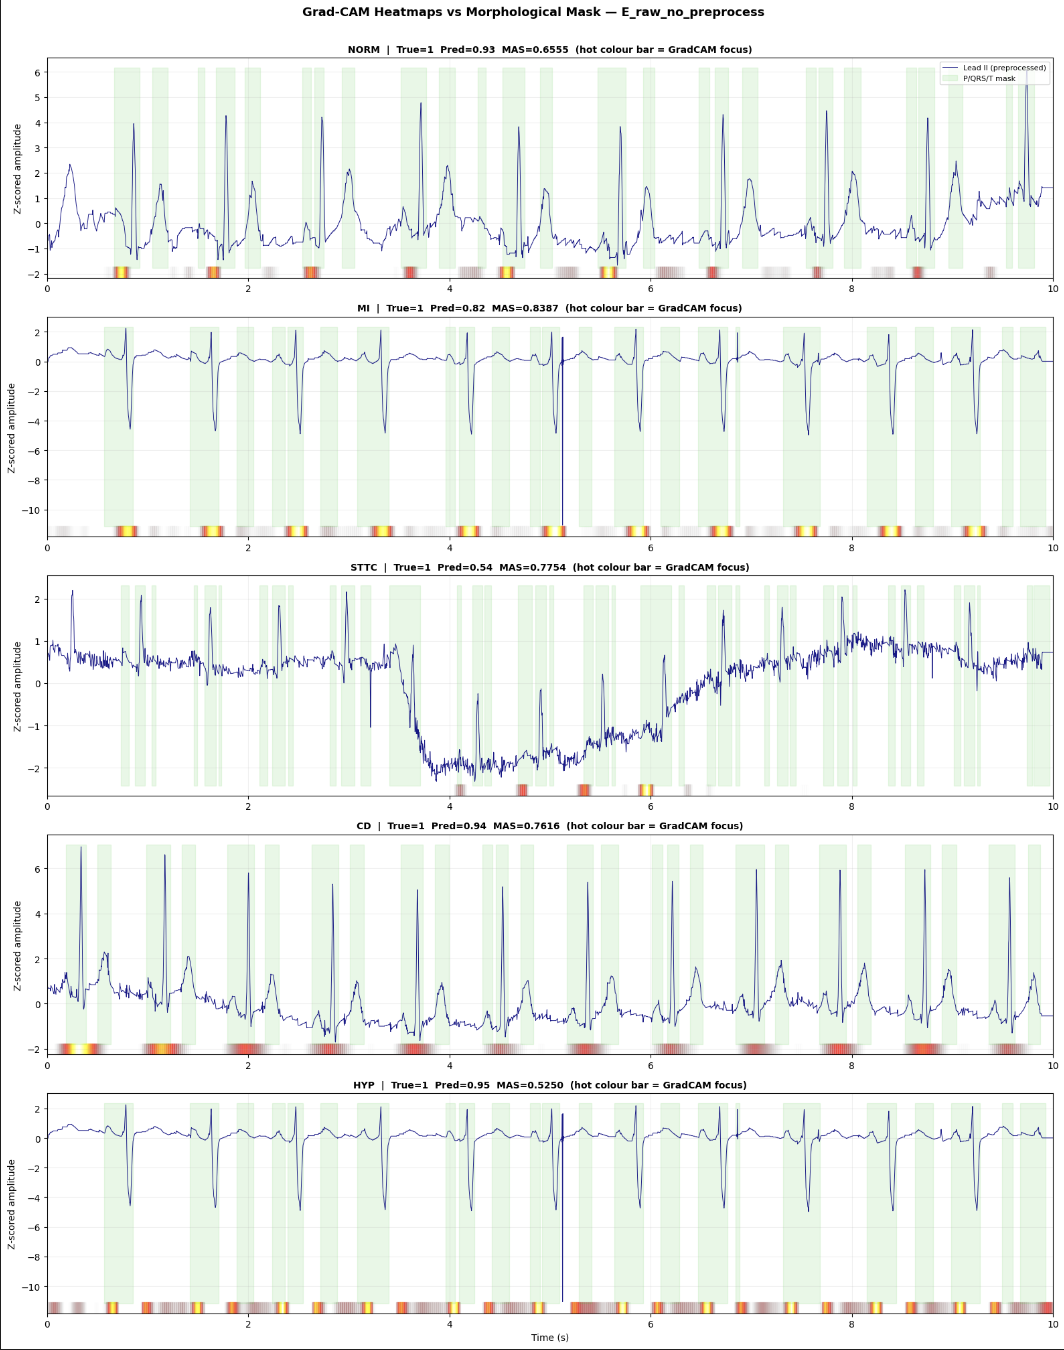
\includegraphics[width=0.78\textwidth]{gradcam_E.png}
\caption{\textbf{Condition E (raw + z-score, no filter) — all five superclasses.}
Same architecture and training procedure as Condition~A; only preprocessing changed.
Per-class MAS\textsubscript{eval}: NORM = 0.656, MI = 0.839, STTC = 0.775,
CD = 0.762, HYP = 0.525 (mean = 0.711). The heatmap colourbar aligns
visibly with the green mask regions across all classes, consistent with the
48\% relative MAS improvement over Condition~A.}
\label{fig:gradcam_E}
\end{figure*}

\begin{table}[h!]
\caption{Per-class MAS\textsubscript{eval} breakdown by condition.}
\label{tab:mas_breakdown}
\vskip 0.1in
\begin{center}
\begin{small}
\begin{tabular}{lrrrrr}
\toprule
Cond. & NORM & MI & STTC & CD & HYP \\
\midrule
A & 0.261 & 0.395 & 0.255 & 0.621 & 0.330 \\
B & 0.281 & 0.770 & 0.604 & 0.392 & 0.812 \\
C & 0.577 & 0.319 & 0.857 & 0.529 & 0.673 \\
D & 0.492 & 0.290 & 0.555 & 0.571 & 0.347 \\
\textbf{E} & \textbf{0.656} & \textbf{0.839} & \textbf{0.775} & \textbf{0.762} & \textbf{0.525} \\
\bottomrule
\end{tabular}
\end{small}
\end{center}
\end{table}

\subsection{Task 5: Physiological Alignment Supervision}

Table~\ref{tab:alignment} reports absolute metrics and
Table~\ref{tab:alignment_delta} shows deltas relative to the
Baseline condition. Note that MAS\textsubscript{physio} values are
not comparable to the MAS\textsubscript{eval} values in Task~4:
they use different masks (Gaussian priors versus binary NeuroKit2)
and are averaged over the full test population rather than
representative samples.

\begin{table}[h!]
\caption{Task~5 alignment ablation. MAS\textsubscript{physio} is the
mean class-specific MAS averaged over the test population. Epochs = 30.}
\label{tab:alignment}
\vskip 0.1in
\begin{center}
\begin{scriptsize}
\begin{tabular}{lrrrr}
\toprule
Ablation & Macro-AUC & Macro-F1 & MAS\textsubscript{physio} & Std \\
\midrule
Baseline   & 0.8960 & 0.6690 & 0.00451 & 0.169 \\
Align      & 0.8964 & 0.6729 & 0.00712 & 0.167 \\
Align$+$Out & 0.8963 & 0.6727 & 0.00713 & 0.152 \\
\textbf{Full} & \textbf{0.8968} & 0.6716 & \textbf{0.00713} & 0.152 \\
\bottomrule
\end{tabular}
\end{scriptsize}
\end{center}
\end{table}

\begin{table}[ht]
\caption{Task~5 deltas relative to Baseline. CD gains most
because QRS widening maps to the narrowest, most precise physiological
prior ($\sigma{=}40$\,ms).}
\label{tab:alignment_delta}
\vskip 0.1in
\begin{center}
\begin{scriptsize}
\begin{tabular}{lrrrrr}
\toprule
Ablation & $\Delta$AUC & $\Delta$F1 & $\Delta$MAS\textsubscript{p} & $\Delta$CD & $\Delta$STTC \\
\midrule
Align      & +.0004 & +.0039 & +.0026 & +.0096 & +.0023 \\
Align$+$Out & +.0003 & +.0037 & +.0026 & +.0094 & +.0024 \\
Full       & +.0008 & +.0026 & +.0026 & +.0097 & +.0023 \\
\bottomrule
\end{tabular}
\end{scriptsize}
\end{center}
\end{table}

The alignment supervision delivers a 58\% relative increase in
mean class-specific MAS (0.00451 to 0.00713) with an AUC gain of
$+0.0008$. The CD class shows the largest absolute gain:
MAS\textsubscript{physio,CD} goes from 0.001 to 0.011 under the
Full condition, roughly a tenfold increase. The effect on HYP is
also positive (0.009 to 0.009 under Align, essentially unchanged).
Classification metrics are well-preserved: the Align condition
actually gives the best Macro-F1 (0.6729 vs 0.6690 for Baseline).

%--------------------------------------------------------------------
\section{Discussion}

\subsection{Why Raw Signal Outperforms Filtered Input}

The most counterintuitive result in this work is that removing all
filtering improves both classification and morphological alignment.
The explanation is not complicated once you look at the fidelity
numbers in Table~\ref{tab:fidelity}. Both Butterworth and SWT retain
only 62--68\% of P-wave amplitude on average. The P-wave sits
predominantly in the 0.5--5\,Hz band; a Butterworth cutoff at 0.5\,Hz
clips that band's lower edge, smoothing the wave. The SWT is better
for R-peak sharpness (97\% retention vs 66\%), but P-wave retention
is nearly identical to Butterworth at 61--68\%. A model trained on
pre-smoothed P-waves cannot be expected to learn P-wave-dependent
patterns reliably, and the Grad-CAM maps confirm this: conditions A
and C both show weak localisation to P-wave regions for CD, the class
most sensitive to P-wave timing.

The raw signal presumably helps because the ResNet can learn to ignore
low-frequency drift (which appears consistently across training
samples) while retaining the full amplitude information of every wave.
Z-score normalisation removes the inter-recording amplitude scale but
leaves intra-recording morphological shape intact.

\subsection{Why LBWA Did Not Help}

We expected LBWA to improve both generalisation and alignment by
exposing the model to more authentic morphological variation while
preserving the P-QRS-T ordering. The opposite happened. There are
a few plausible explanations worth considering.

Piecewise time-warping within validated RR segments may still
introduce subtle distortions at segment boundaries that the
morphological fidelity check does not catch. The model could be
learning to average over these boundary artefacts rather than
sharpening its representation of the beat interior. Alternatively,
LBWA's amplitude perturbation ($a_i \sim \mathcal{N}(1.0, 0.05)$)
at 5\% variation may be enough to confuse the Grad-CAM calibration
used by MAS\textsubscript{eval}, even if the underlying model has
not changed substantially. Either way, the negative result is clear
and consistent across both filtering regimes. We would have needed
to train on substantially more epochs with LBWA or tune $\alpha$
further to say anything more definitive about whether the failure
is fundamental.

\subsection{Alignment Supervision: What Works and What Does Not}

The CD result (tenfold MAS\textsubscript{physio} increase) is the
clearest success story. QRS widening is a spatially compact,
reproducible target: the Gaussian prior for CD centres on $t_R$ with
$\sigma = 40$\,ms, which maps to a narrow 40-sample window at 500\,Hz.
When the alignment loss pushes the CAM toward that window, there is
little ambiguity about where the region is, so the gradient signal is
clean. STTC and MI see smaller gains (per Table~\ref{tab:alignment_delta}),
likely because their ST and T-wave priors overlap spatially and the
multi-label nature of PTB-XL means both labels are often active
simultaneously.

The low absolute values of MAS\textsubscript{physio} (0.007 at best)
reflect the narrowness of the Gaussian priors rather than failure of
alignment. A model attending perfectly to the QRS window would still
produce a low MAS\textsubscript{physio} if the prior is narrow relative
to the signal length. The informative quantity is the relative
improvement, not the absolute score.

Macro-F1 tells a slightly nuanced story: Align has the best F1
(0.6729), while Full (which adds entropy sharpening) has slightly
lower F1 (0.6716) but the best AUC (0.8968). The entropy loss
sharpens localisation at the cost of some probability calibration,
suggesting a tradeoff between spatial precision and class separation
that a more sophisticated schedule might resolve.

%--------------------------------------------------------------------
\FloatBarrier
\section{Conclusion}

Three things emerged clearly from this work.

Butterworth filtering, widely used in ECG deep learning pipelines,
measurably suppresses P-wave amplitude below the threshold needed for
reliable P-wave-dependent learning. Raw ECG with z-score normalisation
is a better starting point for morphological classification on PTB-XL,
and this likely generalises to other clean clinical datasets.

Beat-preserving augmentation designed to simulate physiological heart
rate variability (LBWA) did not improve alignment or accuracy in this
study. Whether this is a fundamental property of beat-warping or a
consequence of our specific implementation and hyperparameter choices
remains open.

Explicitly regularising the model's class activation maps toward
class-specific physiological priors does improve morphological
alignment in a measurable way, with the Conduction Disturbance class
showing the clearest gain. The classification cost is negligible.

Several limitations constrain these findings. The experiment is
restricted to three-lead input in Tasks~4 and~5, which limits the
clinical scope. The physiological priors are defined by fixed offsets
from R-peaks, so records with irregular heart rates or pathological
conduction delays will receive noisy supervision. The MAS metrics
evaluate a single sample per class in Task~4 and narrow Gaussian
windows in Task~5; neither fully captures whether the model reasons
about morphology the way a cardiologist does.

Future work should pursue learnable mask boundaries that adapt to
per-patient conduction velocities, multi-head attention where each
head is supervised toward a distinct wave region, and contrastive
pretraining to push morphologically distinct classes further apart in
feature space. ProtoECGNet~\cite{sethi2025} defines the ceiling for
intrinsic explainability on this dataset; closing the gap between
alignment-supervised models and prototype-based reasoning is the
most natural next step. Furthermore, for greater appeal medical trust and safety standards, we plan on validating the learnt model on various datasets such as the MIT-BIH to ensure that the model is data-agnostic.

%--------------------------------------------------------------------
\clearpage
\bibliography{main}
\bibliographystyle{icml2021}

\end{document}
